% ShadowWeave workshop paper -- full version, NeurIPS 2026 style.
% Default (no option) = SUBMISSION mode: anonymized automatically + line numbers,
% which is what RoboWM's double-blind OpenReview review wants. For the de-anonymized
% camera-ready, switch to \usepackage[final]{neurips_2026}.
\documentclass{article}
\usepackage{neurips_2026}
% \usepackage[final]{neurips_2026}   % camera-ready

\usepackage[utf8]{inputenc}
% NOTE: no [T1]{fontenc} — this TeX Live lacks cm-super/lmodern, so T1 falls back to
% fuzzy bitmap PK fonts; default (OT1) Computer Modern stays fully vector.
\usepackage{graphicx}
\usepackage{booktabs}
\usepackage{amsmath}
\usepackage{microtype}
\usepackage[colorlinks=true,linkcolor=blue,citecolor=blue,urlcolor=blue]{hyperref}

\graphicspath{{../figures/}}

\title{ShadowWeave: A Calibrated World Model of Occluded Space from a Single Depth Frame}

% The style file anonymizes this automatically in submission mode.
\author{Kushaan Naskar\\
  University of Massachusetts Amherst\\
  \texttt{kushaannaskar@gmail.com}}

\begin{document}

\maketitle

\begin{abstract}
An embodied agent must model the physical scene it cannot directly see --- the occupancy occluded
by the walls and obstacles it moves among (``shadow''). A world model that represents only the
visible surface is blind to half its workspace. We study how well a model can
\textbf{complete} occupancy in that occluded region from a \textbf{single monocular-depth frame}, and,
crucially, whether it knows \emph{when it is guessing}. ShadowWeave projects one depth frame into an
egocentric bird's-eye-view (BEV) occupancy grid, marks the unobserved cells with an explicit
shadow mask, and predicts occupancy inside that mask together with a per-cell uncertainty. On a
MuJoCo indoor benchmark, the model beats a persistence baseline by a micro-averaged shadow-IoU
gain of \textbf{+0.31 to +0.36 at a 5\,s horizon} (95\% per-episode bootstrap CIs clear of zero at
every horizon), far exceeds an observation-blind dataset prior even at the prior's best threshold
(0.61--0.72 IoU vs 0.08--0.10), and its uncertainty is \textbf{better calibrated inside shadow
(ECE 0.043--0.047, at 5\,s) than in directly observed space (0.058--0.086)}. We frame prediction
into occluded space as \textbf{world modeling of the unobserved physical scene} --- inferring the
occupancy state a downstream controller needs where the sensor has no view --- and introduce a
decomposition that separates \emph{amodal completion} of persistent hidden structure from
\emph{temporal forecasting} of dynamics. It yields an honest characterization of this single-frame
world model: its predictive power is almost entirely spatial completion --- the pure-forecasting
residual is small ($\le$+0.007 at 5\,s) and decays with horizon. Randomizing room geometry per
episode leaves the gain statistically unchanged on rooms the model never saw, ruling out
memorization of a fixed room shell. The completion path runs at 7\,ms (p95), well inside a 20\,Hz
control budget; end-to-end with an off-the-shelf monocular-depth network it runs at ${\sim}18$\,Hz
on 2017-era hardware. The completed grid and its uncertainty feed an eyes-free spatial-audio
navigation interface as a systems demonstration. We release the evaluation methodology --- an
empty-credit-immune micro-averaged gain, a completion/forecasting decomposition, and per-episode
confidence intervals --- as a reusable protocol for honest occupancy-completion claims.
\end{abstract}

\section{Introduction}
\label{sec:intro}

Any embodied agent acting in the physical world must reason about the parts of a scene it cannot
directly observe --- the occupancy occluded by the very walls and obstacles it moves among. A
world model that represents only what the sensor sees is blind to half of the workspace: a robot
rounding a shelf, an agent entering a room, a planner routing around a blind corner all depend on
the \emph{unobserved} physical state as much as the visible one, and completing that hidden state
is a prerequisite for reasoning about what happens next. Sensing provides a partial view; the rest
must be inferred, and for any downstream use --- planning, control, or a human-facing interface ---
that inference is only trustworthy if it carries an honest estimate of its own reliability: a
confident hallucination of clear space behind a wall is worse than a calibrated ``I don't know.''

Prior work addresses parts of this problem but not their conjunction. Semantic scene completion,
from MonoScene \citep{cao2022monoscene} through VoxFormer \citep{li2023voxformer} and
VisHall3D \citep{lu2025vishall3d}, hallucinates dense geometry beyond the visible
frontier from a single image, but targets outdoor driving voxels scored by mIoU alone, with no
notion of calibrated confidence in the hallucinated region. Occupancy world models such as
OccWorld \citep{zheng2024occworld} forecast the \emph{temporal} evolution of multi-frame occupancy for autonomous driving.
Closest to our setting, ProxMaP \citep{sharma2023proxmap} completes indoor proximal occupancy from a single top-down view
to improve navigation --- but it emits a point estimate, with no explicit occlusion mask, no
calibrated uncertainty in the hidden cells, and no attribution of \emph{where} its predictive power
comes from.

We present \textbf{ShadowWeave}, a world model of occluded space: from a single monocular-depth
frame it produces (i) an egocentric BEV occupancy grid, (ii) an explicit shadow mask marking the
cells the sensor cannot see, and (iii) a calibrated per-cell occupancy probability inside that
mask. Unlike occupancy world models built for temporal forecasting, it models the \emph{unobserved
present} --- the state behind obstacles --- and we quantify exactly how much of its predictive
power is spatial completion versus temporal forecasting. We evaluate it with a
protocol designed to resist the standard failure modes of occupancy metrics: an
empty-credit-immune, micro-averaged shadow-IoU gain over a persistence baseline; per-episode
bootstrap confidence intervals; and a static/dynamic/never decomposition that attributes the gain
to \emph{completion} of persistent hidden structure versus \emph{forecasting} of dynamics. Downstream, the
completed grid and its uncertainty feed an A* planner and a nine-zone HRTF spatial-audio
interface for eyes-free navigation, which we include as a systems demonstration.

Our contributions are:

\begin{itemize}
\item \textbf{A calibrated amodal-completion result.} From one depth frame, the model completes occluded
  occupancy with a micro-averaged shadow gain of +0.31--0.36 at 5\,s (CIs clear of zero at every
  horizon), and its in-shadow uncertainty is \emph{better} calibrated (ECE 0.043--0.047 at 5\,s) than in
  observed space.
\item \textbf{A decomposition methodology} that separates completion from forecasting. It reveals that the
  gain is spatial completion of persistent hidden structure; the pure-forecasting residual is
  at or near zero (fixed static +0.000; moving tier +0.007 [+0.002, +0.012] at 5\,s --- statistically
  significant but practically small, and decaying with horizon as real forecasting should). We
  report this negative honestly: most pooled occupancy numbers in the literature are vulnerable to
  exactly the confound this decomposition dissects.
\item \textbf{A memorization confound-kill.} Randomizing room geometry per episode leaves the gain
  statistically unchanged on never-seen rooms (+0.306 fixed vs +0.309 [+0.294, +0.324]
  randomized), showing the completion is per-scene inference, not a memorized constant layout.
\item \textbf{A real-time completion front-end.} The completion path runs at 7\,ms p95 (well inside
  a 20\,Hz budget); end-to-end with an off-the-shelf monocular-depth network it is ${\sim}18$\,Hz on
  2017-era hardware. Its output feeds an A* + nine-zone HRTF eyes-free interface, which we present
  as a systems demonstration (it does not yet meet navigation collision targets; \S\ref{sec:system}).
\end{itemize}

\section{Method}
\label{sec:method}

\begin{figure}[t]
  \centering
  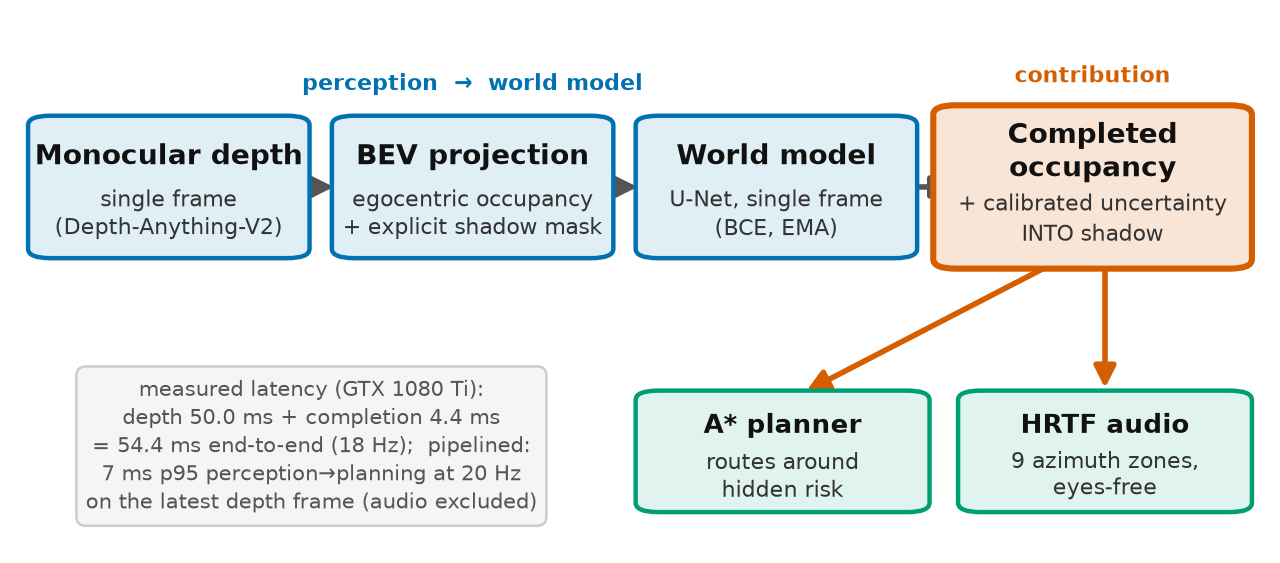
\includegraphics[width=0.92\linewidth]{architecture.png}
  \caption{ShadowWeave pipeline. A single monocular-depth frame is lifted into an egocentric
  $96\times96$ BEV occupancy grid plus a visibility grid; thresholding visibility yields the shadow
  mask. A 31M-parameter U-Net completes per-cell occupancy at 1/3/5/10\,s inside the mask; the
  completed grid and its uncertainty feed an A* planner and a nine-zone HRTF audio interface
  (system context).}
  \label{fig:architecture}
\end{figure}

\subsection{From a depth frame to an egocentric BEV with a shadow mask}
\label{sec:bev}

At each step the agent observes a single monocular-depth image (in simulation, the renderer's
depth; in deployment, a monocular-depth network such as Depth-Anything-V2-Small). A differentiable
projector lifts the depth map into an egocentric bird's-eye-view (BEV) occupancy grid of size
$96\times96$ covering 5\,m ahead, together with a \textbf{visibility} grid: cells along a ray up to the first
returned surface are marked observed-free, the surface cell observed-occupied, and everything
beyond the surface \textbf{shadow} --- geometry the sensor cannot see. Thresholding visibility at 0.5
yields the binary shadow mask that defines the region of interest for every metric in this paper
(Fig.~\ref{fig:architecture}).
Optical flow between consecutive BEV frames provides an optional motion channel.

\subsection{World model}
\label{sec:worldmodel}

We treat the network as a \textbf{world model of occluded space}: it infers the environment's
occupancy state where the sensor has no view, rather than only labeling what is directly measured.
Its predictive power, as \S\ref{sec:completion} quantifies, concentrates in spatial completion of
persistent hidden structure rather than temporal forecasting of dynamics --- a property of this
single-frame model class, made measurable by our decomposition. A U-Net (31M parameters) takes the
single-frame BEV stack and predicts occupancy at horizons of 1, 3, 5, and 10\,s as per-cell
probabilities. It is trained with binary cross-entropy (positive
class up-weighted, since BEV targets are $\approx$7\% occupied) on 400 training episodes, with early
stopping and exponentially-averaged (EMA) weights; we report the epoch-8 checkpoint (validation
loss 0.300, validation IoU@5s 0.665). Ablations (\S\ref{sec:ablations}) show the visibility and flow channels are
redundant --- the completion signal is carried by the occupancy channel alone --- so the deployable
model reduces to depth$\to$occupancy$\to$completion. The input is a \textbf{single frame}: the model has no
multi-frame memory, which is what makes the completion-vs-forecasting distinction (\S\ref{sec:decomp}) sharp.

\subsection{Uncertainty in shadow}
\label{sec:uncertainty}

The model's per-cell occupancy probability \emph{is} its uncertainty estimate; the claim we test in
\S\ref{sec:calibration} is that this probability is \textbf{calibrated inside the shadow region specifically}, not merely
grid-wide (where easy free space dominates). Calibrating uncertainty in the occluded region is the
property that makes the output safe to consume downstream.

\subsection{Downstream eyes-free interface (system context)}
\label{sec:interface}

The completed occupancy grid and its uncertainty drive an A* global planner (which owns
goal-seeking and pays an extra cost to route through unobserved cells) and a reactive local
collision-avoidance policy. Occupancy and uncertainty in nine azimuth zones are rendered as
HRTF-spatialized audio cues for eyes-free navigation. We describe this interface for context and
report its latency and navigation behavior honestly (\S\ref{sec:system}); the audio interface itself is a
system demonstration, not a user-evaluated result.

\section{Evaluation methodology}
\label{sec:methodology}

Occupancy metrics are easy to report and easy to inflate. Because our claim lives entirely inside
a sparse, mostly-empty sub-region (shadow is ${\sim}$92\% never-occupied), we adopt a protocol built to
resist the specific ways such a claim can look better than it is. We consider this protocol a
contribution in its own right.

\subsection{The empty-credit trap and micro-averaging}
\label{sec:microavg}

The natural masked IoU scores an empty prediction against an empty masked region as a perfect 1.0
(``correctly predicted nothing here''). Since most shadow cells are legitimately empty, this inflates
both the model and the baselines, and the inflation is not uniform across sub-masks. We therefore
report \textbf{micro-averaged} shadow IoU: pool integer intersection and union counts across all frames
and divide once, so rare sub-masks cannot each contribute a free 1.0. Empty denominators report as
undefined, never as 1.0. The defended quantity is the \textbf{gain} over a persistence baseline (the
observed frame carried forward), not the absolute level.

\subsection{Completion vs.\ forecasting decomposition}
\label{sec:decomp}

Within the shadow mask, we classify each cell by its occupancy pattern across the prediction
horizons --- valid because all horizons are rendered from the same issue pose, so static geometry
projects to identical cells at every horizon:

\begin{itemize}
\item \textbf{STATIC} --- occupied at \emph{all} horizons: persistent hidden structure (walls, static obstacles,
  settled debris); $\approx$7\% of shadow. Recall here measures \textbf{amodal completion}.
\item \textbf{DYNAMIC} --- occupied at \emph{some but not all} horizons: transient-in-window structure (arrivals,
  departures, pass-throughs); $\le$1.5\% of shadow. IoU here measures genuine \textbf{forecasting} beyond
  persistence.
\item \textbf{NEVER} --- occupied at \emph{no} horizon: free hidden space; $\approx$92\% of shadow. The false-positive
  test.
\end{itemize}

One caveat follows from the sampling: because the split keys on the four rendered horizons
$\{1, 3, 5, 10\}$\,s, dynamics faster than the 1\,s grid --- e.g.\ debris that is aloft and settles
within the first second --- are absorbed into STATIC, which biases the split toward completion. The
moving tier, whose obstacles are in continuous motion across the whole window, is therefore the
cleaner test of forecasting, and it still shows only a small dynamic gain (\S\ref{sec:completion});
a finer horizon grid is future work.

Reporting completion and forecasting separately is what lets us state honestly that the gain is
completion, not clairvoyance --- a distinction the pooled shadow-IoU hides.

\subsection{Per-episode bootstrap confidence intervals}
\label{sec:bootstrap}

Frames within an episode share geometry and pose and are correlated, so resampling frames would
understate uncertainty. We resample \textbf{episodes} with replacement ($B = 10{,}000$), recompute the
pooled micro-gain per replicate, and take the paired model-minus-persistence difference within each
replicate (the two are positively correlated across episodes). We report the resulting 2.5/97.5
percentile interval for every headline gain.

\subsection{Calibration in shadow}
\label{sec:calib-method}

We measure expected calibration error (ECE) restricted to shadow cells, contrasted with observed
cells and with a walls-excluded variant, using equal-mass binning (a fine 1000-bin histogram merged
into 15 equal-count macro-bins, because in-shadow probabilities cluster near the prior and
equal-width bins would be mostly empty). ECE-in-shadow close to or below ECE-in-observed is the
evidence that uncertainty propagates faithfully into unseen space.

\section{Experiments}
\label{sec:experiments}

\subsection{Setup}
\label{sec:setup}

We use a MuJoCo single-room benchmark with three difficulty tiers --- \textbf{static} (fixed obstacles),
\textbf{moving} (kinematically driven movers), and \textbf{debris} (objects that fall and settle) --- with 400
training and 80 validation episodes on disjoint seeds; the per-tier decomposition and CI
analyses use clean single-tier validation sets of 30 episodes (9{,}000 frames) each, and the
randomized-geometry validation (\S\ref{sec:robustness}) uses 80 episodes. The BEV is $96\times96$ over 5\,m; horizons are
1/3/5/10\,s. Unless noted, fixed-geometry results use a $6\times6$\,m room; \S\ref{sec:robustness} randomizes geometry.
Reproducibility is pinned: the fixed-geometry scene generation is verified bit-exact against a
golden hash, and a full rollout re-run reproduces every accuracy metric bit-identically
(wall-clock latency, which is hardware-dependent, is the one exception).

\subsection{Shadow-gain headline}
\label{sec:headline}

The model predicts occupancy in cells the sensor cannot see, beating persistence at every horizon.
Micro-averaged shadow gain at 5\,s, per tier, with 95\% bootstrap CIs, is shown in
Table~\ref{tab:gain}.

\begin{table}[t]
  \centering
  \caption{Micro-averaged shadow-IoU gain over the persistence baseline at the 5\,s horizon on the
  fixed-geometry validation set, per tier, with 95\% per-episode bootstrap confidence intervals.}
  \label{tab:gain}
  \begin{tabular}{lcc}
    \toprule
    tier (fixed val, @5\,s) & micro shadow gain & 95\% CI \\
    \midrule
    static & +0.306 & [+0.288, +0.327] \\
    moving & +0.363 & [+0.349, +0.378] \\
    debris & +0.315 & [+0.281, +0.350] \\
    \bottomrule
  \end{tabular}
\end{table}

\begin{figure}[t]
  \centering
  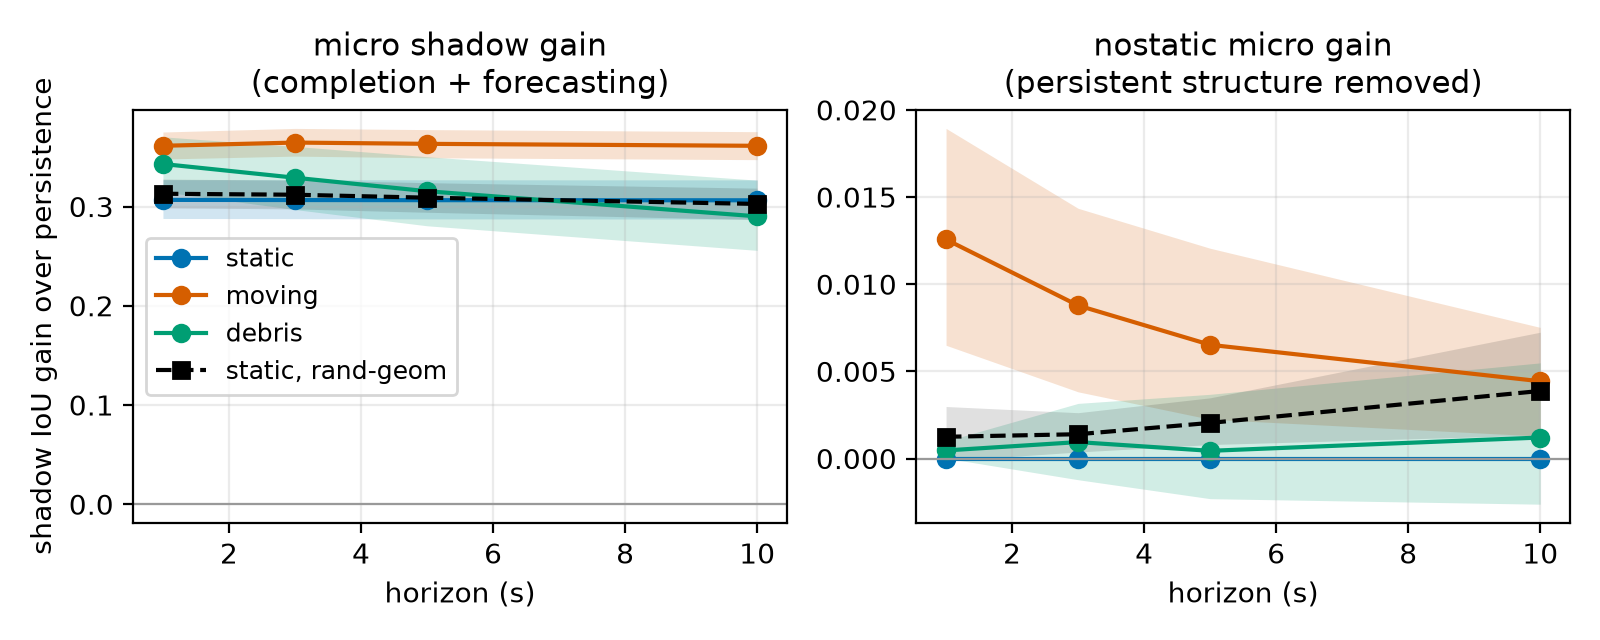
\includegraphics[width=0.9\linewidth]{shadow_gain_ci.png}
  \caption{Micro-averaged shadow-IoU gain over persistence per tier and horizon, with 95\%
  per-episode bootstrap confidence intervals. Every interval is clear of zero at every horizon,
  so the gain is statistically significant rather than sampling noise.}
  \label{fig:shadowgain}
\end{figure}

Every interval is clear of zero at every horizon, so the gain is statistically significant rather
than sampling noise (Fig.~\ref{fig:shadowgain}; all horizons tabulated in
Appendix~\ref{app:gains}). In policy rollouts the frame-averaged (macro)
shadow gain is +0.325\slash+0.322\slash+0.320\slash+0.178 at 1/3/5/10\,s. (Raw macro shadow-IoU levels --- model 0.744 vs
persistence 0.424 at 5\,s --- are empty-credit inflated and are reported only for reference; the
micro-gain is the defended number.)

\paragraph{Beyond persistence.} Persistence could be a weak baseline for \emph{completion}, so we
test two stronger ones (full tables in Appendix~\ref{app:prior}). An observation-blind
pose-marginal prior (mean training occupancy, swept to its best threshold) reaches only
0.08--0.10 micro shadow IoU: it recalls hidden structure (0.86--0.92) only by blanketing 72--79\%
of empty hidden space with false positives, whereas the model achieves 0.61--0.72 IoU at a
1.4--3.4\% false-positive rate. An observation-conditioned dilation heuristic peaks at micro
shadow IoU 0.31--0.35, at or below persistence itself. Hidden structure is thus non-local:
copying the observation, extrapolating it locally, and an observation-blind prior all fail.
Together with the geometry-randomization result (\S\ref{sec:robustness}), this rules out
memorized layouts, memorized marginals, and trivial extrapolation alike.

\subsection{What the gain is: completion, not clairvoyance}
\label{sec:completion}

Decomposing the shadow mask (\S\ref{sec:decomp}) attributes the gain almost entirely to amodal completion of
persistent hidden structure (Table~\ref{tab:decomp}, Fig.~\ref{fig:decomp}).

\begin{table}[t]
  \centering
  \caption{Completion/forecasting decomposition of the shadow mask on the fixed-geometry
  validation set at 5\,s (dynamic IoU rows span the 1\,s$\to$10\,s horizons). The gain is carried
  by recall of persistent hidden structure (amodal completion), not by forecasting of dynamics.}
  \label{tab:decomp}
  \begin{tabular}{lcc}
    \toprule
    component (fixed val @5\,s) & model & persistence \\
    \midrule
    persistent-structure recall (amodal completion) & 0.83--0.93 & 0.37--0.51 \\
    dynamic IoU, moving tier (1\,s$\to$10\,s) & 0.092 $\to$ 0.031 & 0.060 $\to$ 0.020 \\
    dynamic IoU, debris tier & 0.020 $\to$ 0.019 & 0.006 $\to$ 0.023 \\
    false-positive rate on never-occupied cells & 0.014--0.034 & 0.022--0.027 \\
    \bottomrule
  \end{tabular}
\end{table}

\begin{figure}[t]
  \centering
  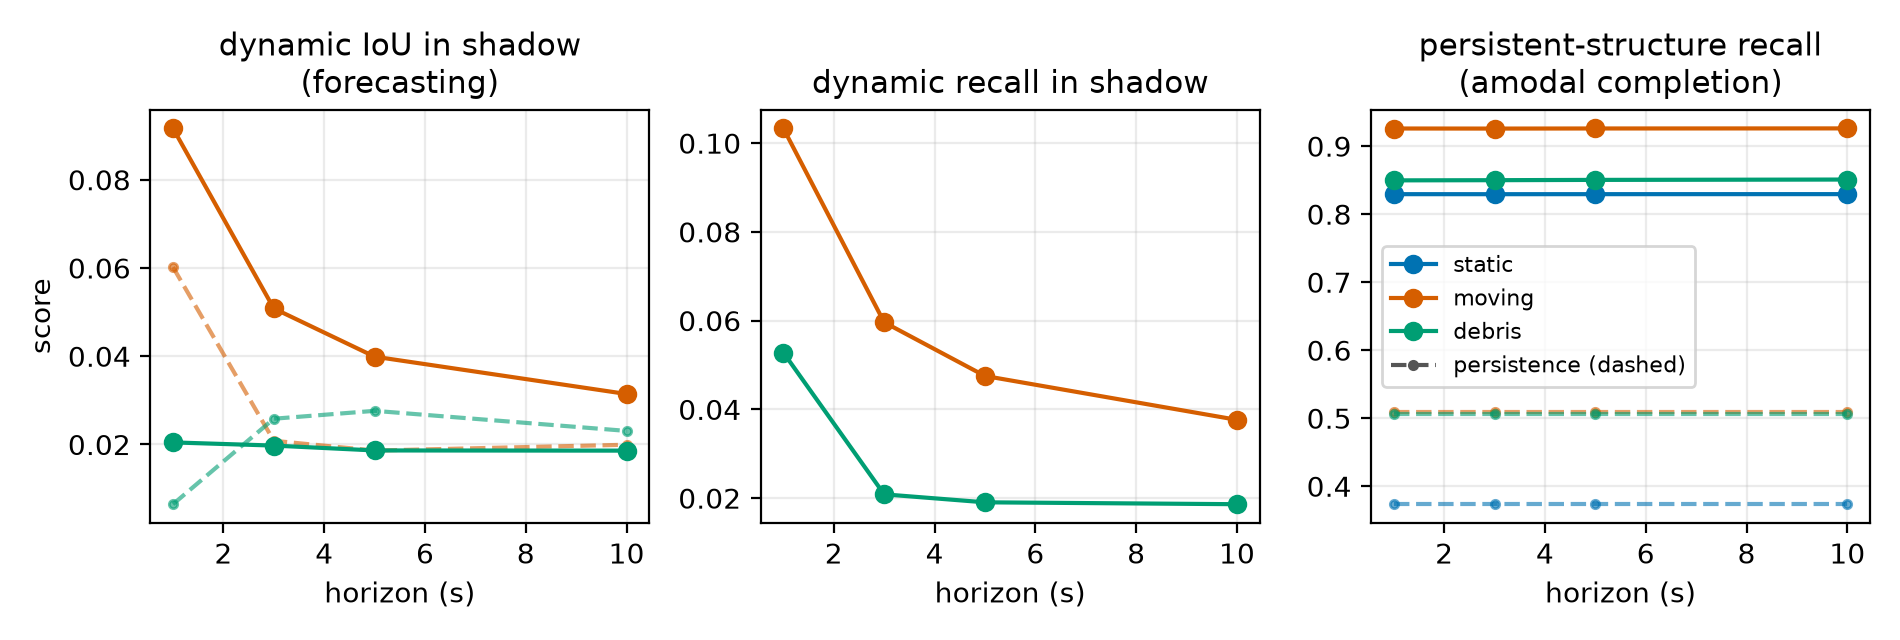
\includegraphics[width=0.97\linewidth]{decomp_curves.png}
  \caption{Decomposition of the shadow gain across horizons: persistent-structure recall (amodal
  completion) versus dynamic IoU (forecasting) for model and persistence. The gain is spatial
  completion of persistent hidden structure; the small dynamic-forecasting signal on the moving
  tier decays with horizon as genuine forecasting should.}
  \label{fig:decomp}
\end{figure}

Excluding all persistent structure, the residual ``nostatic'' gain is at or near zero: fixed
static +0.000, moving +0.007 (CI [+0.002, +0.012]), randomized-geometry static +0.002
([+0.001, +0.004]) at 5\,s. The honest claim is therefore \textbf{amodal completion of hidden
structure}, with a small but statistically significant dynamic-forecasting signal on the moving
tier that decays with horizon as genuine forecasting should. We do not claim dynamic forecasting on
debris, where the dynamic signal is at the noise floor and persistence matches the model beyond
1\,s.

\subsection{Robustness to room geometry (memorization confound-kill)}
\label{sec:robustness}

A fixed room shell could let the model memorize a constant wall prior. We regenerated the data with
per-episode randomized room width and depth (each drawn i.i.d.\ in $[5, 8]$\,m, obstacle counts scaled
to hold the ${\sim}$7\% positive fraction), retrained the model from scratch, and evaluated on 80 held-out
randomized rooms (Table~\ref{tab:randomized}).

\begin{table}[t]
  \centering
  \caption{Static-tier shadow gain at 5\,s under fixed versus per-episode randomized room
  geometry. The gain does not drop on never-seen rooms, ruling out memorization of a constant
  layout.}
  \label{tab:randomized}
  \begin{tabular}{lccc}
    \toprule
    static tier, @5\,s & micro shadow gain & 95\% CI & completion recall \\
    \midrule
    fixed $6\times6$ geometry & +0.306 & [+0.288, +0.327] & 0.829 \\
    \textbf{randomized geometry} & \textbf{+0.309} & \textbf{[+0.294, +0.324]} & 0.854 \\
    \bottomrule
  \end{tabular}
\end{table}

The gain does not drop --- the intervals overlap almost entirely, and completion recall is if
anything slightly higher on never-seen rooms. Memorizing a constant shell contributes essentially
nothing; completion is per-scene inference.

\subsection{Calibration in shadow}
\label{sec:calibration}

Shadow is ${\sim}$92\% empty, so a raw in-shadow ECE is easy to make small --- probability mass
clusters near the prior. We therefore lead with the harder number: \emph{excluding the persistent
structure entirely} (the walls and settled cells that dominate the mask), in-shadow ECE at 5\,s
remains a low 0.055--0.056 on the tiers with dynamic content (on the static tier the
structure-excluded region has no positive labels, so no calibration curve exists there).
Calibration is thus carried by the genuinely uncertain cells, not the easy always-occupied ones.
On the full shadow mask at 5\,s, in-shadow ECE is 0.043--0.047 across tiers --- lower than in
observed space (0.058--0.086), with Brier 0.022--0.036 (Fig.~\ref{fig:reliability}) --- though we
note this shadow-vs-observed edge is aided by shadow's emptiness and is a secondary observation,
not the primary claim. The model is underconfident in the mid-range but places little mass there.
Calibration is not an artifact of the fixed room: on randomized geometry, in-shadow ECE is
0.050--0.067 vs observed 0.056--0.077, with shadow the better-calibrated region only at the longer
5--10\,s horizons (at 1\,s the two are comparable). The reliability diagram is in
Appendix~\ref{app:reliability} (Fig.~\ref{fig:reliability}).

\subsection{Ablations: occupancy alone carries the signal}
\label{sec:ablations}

Dropping either auxiliary input channel and retraining leaves the gain intact
(Table~\ref{tab:ablations}).

\begin{table}[t]
  \centering
  \caption{Input-channel ablations. Shadow gain at 5\,s (micro, per tier) and rollout shadow gain
  at 5\,s for the full model and the no-visibility and no-flow variants.}
  \label{tab:ablations}
  \small
  \setlength{\tabcolsep}{4pt}
  \begin{tabular}{lcc}
    \toprule
    variant & \begin{tabular}[c]{@{}c@{}}shadow gain @5\,s\\ (micro, static/moving/debris)\end{tabular} & rollout shadow gain @5\,s \\
    \midrule
    full (occupancy+visibility+flow) & +0.306 / +0.363 / +0.315 & +0.320 \\
    no visibility & +0.309 / +0.360 / +0.313 & --- \\
    no flow & --- & +0.381 \\
    \bottomrule
  \end{tabular}
\end{table}

The no-visibility per-tier gains are within CI of the full model; the no-flow rollout gain is if
anything higher. Both auxiliary channels are redundant, which simplifies the input and removes
optical-flow estimation from the runtime critical path. These independently retrained variants
also bound training-run variance: every one of them (and the separately trained
randomized-geometry model of \S\ref{sec:robustness}) lands within the full model's per-tier
confidence intervals, so the headline gain is not an artifact of a lucky training seed.

\subsection{System: latency and navigation}
\label{sec:system}

\paragraph{Latency.} The perception-to-planning path (BEV projection, raycaster, world-model
forward, orchestrator; batch 1, deterministic U-Net) runs at 6.47\,ms p50 / 6.99\,ms p95 --- well
inside a 50\,ms (20\,Hz) budget. Depth is the bottleneck: Depth-Anything-V2-Small alone takes
49.9\,ms p50 on the evaluation-era GPU (GTX~1080~Ti, $480{\times}640$), so the sequential
end-to-end pipeline is 54.4\,ms (18\,Hz). A deployed system runs depth asynchronously at its own
rate while the 7\,ms completion path consumes the latest depth frame; audio synthesis is excluded.

We also probed whether the model flags occupancy that materializes in shadow before it is
revealed. Because that metric conflates falling objects with static geometry revealed by agent
motion and does not meet its lead-time target, we report it only as a diagnostic in
Appendix~\ref{app:falling}, not as a result or a contribution.

\paragraph{Navigation.} With the completed grid feeding the planner, the trained reactive policy achieves a
per-episode collision rate of 0.367 (vs 0.60 untrained) and path straightness 0.773, but does not
meet the $\le$0.10 collision target. We present navigation as an honest system demonstration.

A generative (conditional-diffusion) variant of the world model is deferred to
Appendix~\ref{app:generative}.

\section{Related work}
\label{sec:related}

Predicting the structure of unobserved space has been approached from three angles. Semantic scene
completion, from SSCNet \citep{song2017sscnet} through MonoScene \citep{cao2022monoscene} and its
monocular successors VoxFormer \citep{li2023voxformer} and VisHall3D \citep{lu2025vishall3d},
infers dense voxel geometry --- and even
hallucinates geometry beyond the visible frontier --- from a single image, but targets outdoor
driving voxels evaluated purely by mIoU/IoU, without calibrated uncertainty in the occluded region.
Occupancy world models such as OccWorld \citep{zheng2024occworld}, together with occupancy-forecasting
benchmarks (Occ3D; \citealp{tian2023occ3d}) and self-supervised raycasting forecasters
\citep{khurana2023pointcloud}, instead predict the \emph{temporal} evolution of multi-frame occupancy for autonomous vehicles.
Closest in spirit, ProxMaP \citep{sharma2023proxmap} completes indoor proximal occupancy from a single
view for navigation, yet emits only point estimates. ShadowWeave is distinct in delivering
egocentric BEV amodal completion into explicitly masked occluded space from a single
monocular-depth frame, with calibrated uncertainty inside the hidden region, and a
completion-versus-forecasting decomposition showing the gain is spatial completion rather than
dynamics.

\section{Limitations}
\label{sec:limitations}

Our evaluation is in simulation on the simulator's clean depth: ground-truth occluded occupancy is
unavailable on real footage without instrumentation, so no quantitative real-world claim is made
and robustness of the completion to estimated-depth noise is untested, though the front-end accepts
real monocular depth (Depth-Anything-V2). We compare against strong self-constructed baselines
rather than prior methods, which target different input regimes (e.g., ProxMaP's top-down RGB-D
view); a head-to-head on a shared benchmark is future work. Our results characterize a single 31M
single-frame CNN, so the forecasting-negative applies to this model class, not necessarily to
larger or recurrent ones (the evaluation protocol itself is architecture-agnostic). Navigation
does not meet its collision target and the audio interface is not user-evaluated; both are system
context.

\section{Conclusion}
\label{sec:conclusion}

Calibrated amodal completion of occluded occupancy is achievable from a single monocular-depth
frame, transfers to room geometries the model never saw, and can be delivered within a real-time
perception-to-planning budget for an eyes-free interface. Equally important is \emph{how} we measure it:
an empty-credit-immune micro-gain, per-episode confidence intervals, and a decomposition that
separates completion from forecasting keep the claim honest and expose exactly where the predictive
power lies. We hope the protocol is reused: many occupancy-completion results would read differently
under it.

\bibliographystyle{plainnat}
\bibliography{references}

\appendix

\section{Per-horizon shadow gains with confidence intervals}
\label{app:gains}

Table~\ref{tab:gains-full} reports the micro-averaged shadow-IoU gain over persistence at every
horizon, with 95\% per-episode bootstrap confidence intervals (10{,}000 resamples, paired
model$-$persistence). Every interval is clear of zero. The static-tier gain is flat across
horizons (persistent structure does not move); the debris-tier gain decays with horizon as more
debris settles into persistent structure; the randomized-geometry run tracks the fixed-geometry
static tier throughout.

\begin{table}[ht]
  \centering
  \scriptsize
  \setlength{\tabcolsep}{3.5pt}
  \caption{Micro shadow gain over persistence, all horizons, 95\% bootstrap CIs over episodes.}
  \label{tab:gains-full}
  \begin{tabular}{lcccc}
    \toprule
    tier & 1\,s & 3\,s & 5\,s & 10\,s \\
    \midrule
    static & +0.307 [+0.288, +0.327] & +0.307 [+0.288, +0.327] & +0.306 [+0.288, +0.327] & +0.306 [+0.287, +0.327] \\
    moving & +0.361 [+0.348, +0.375] & +0.364 [+0.351, +0.379] & +0.363 [+0.349, +0.378] & +0.361 [+0.347, +0.375] \\
    debris & +0.343 [+0.315, +0.370] & +0.329 [+0.297, +0.361] & +0.315 [+0.281, +0.350] & +0.290 [+0.256, +0.327] \\
    rand.\ geometry & +0.313 [+0.299, +0.328] & +0.312 [+0.298, +0.327] & +0.309 [+0.294, +0.324] & +0.303 [+0.287, +0.318] \\
    \bottomrule
  \end{tabular}
\end{table}

\section{Heuristic baselines: observation-blind prior and dilation}
\label{app:prior}

The pose-marginal prior is the mean training-set occupancy grid in the egocentric frame,
thresholded at whichever of eight thresholds (0.02--0.5) maximizes its micro shadow IoU --- the
most favorable possible reading. Table~\ref{tab:prior} shows that even so, the prior can reach
high structure recall only by blanketing ${\sim}72$--79\% of genuinely empty hidden space with
false positives, capping its IoU at 0.08--0.10 versus the model's 0.61--0.72. One caution:
the prior's IoU restricted to \emph{dynamic} cells should never be quoted in isolation ---
at its best threshold the prior carpet-bombs the dynamic region too, which is meaningless at a
72\% false-positive rate.

\begin{table}[ht]
  \centering
  \small
  \caption{Observation-blind prior at its best threshold (0.05) vs the model, @5\,s.}
  \label{tab:prior}
  \begin{tabular}{lcccc}
    \toprule
    tier & prior micro IoU & prior structure recall & prior FP on empty & model (IoU @ FP) \\
    \midrule
    static & 0.102 & 0.879 & 0.723 & 0.610 @ 0.034 \\
    moving & 0.080 & 0.865 & 0.722 & 0.723 @ 0.015 \\
    debris & 0.089 & 0.869 & 0.717 & 0.670 @ 0.014 \\
    rand.\ geometry & 0.087 & 0.921 & 0.793 & 0.655 @ 0.021 \\
    \bottomrule
  \end{tabular}
\end{table}

The observation-\emph{conditioned} counterpart --- binary dilation of the observed occupancy by
$r \in \{1,\dots,6\}$ cells (one cell ${\approx}10$\,cm), reported at the IoU-maximizing radius
--- probes whether local extrapolation of the observation suffices. It does not
(Table~\ref{tab:dilate}): the heuristic peaks at $r{=}1$, essentially tied with or below plain
persistence, because at matched false-positive rates it recalls only 0.42--0.56 of hidden
structure versus the model's 0.83--0.93, and every larger radius grows false positives faster
than recall, monotonically lowering IoU.

\begin{table}[ht]
  \centering
  \small
  \caption{Observation-conditioned dilation heuristic at its best radius ($r{=}1$) vs
  persistence and the model, micro shadow IoU @5\,s.}
  \label{tab:dilate}
  \begin{tabular}{lcccc}
    \toprule
    tier & dilation (best $r$) & dilation recall @ FP & persistence & model \\
    \midrule
    static & 0.305 & 0.416 @ 0.035 & 0.303 & 0.610 \\
    moving & 0.346 & 0.557 @ 0.039 & 0.360 & 0.723 \\
    debris & 0.342 & 0.544 @ 0.039 & 0.355 & 0.670 \\
    \bottomrule
  \end{tabular}
\end{table}

\section{Occupancy-arrival diagnostic (not falling-object anticipation)}
\label{app:falling}

We keep this out of the main results because it does not measure what a ``falling-object'' metric
should: events are counted per due prediction (one object aloft is scored at every issue step and
horizon it is due, not once per physical object); an ``arrival'' keys on unobserved-at-issue
rather than newly-occupied cells, so occluded \emph{static} geometry revealed by agent motion is
also counted, and the metric pools all tiers; and lead time is bounded by the discrete
$\{1,3,5,10\}$\,s horizon grid, so the $\ge$3\,s target is neither met nor meaningfully measurable
at this granularity. We report it only to characterize the model's behavior, not as a capability
claim.

\begin{table}[ht]
  \centering
  \small
  \caption{Cell-level vs connected-component scoring of the revealed-occupancy proxy.}
  \label{tab:falling}
  \begin{tabular}{lcc}
    \toprule
    metric & cell-level & component-level \\
    \midrule
    detection rate & 0.787 & 0.752 \\
    false-alarm rate & 0.021 & 0.286 \\
    precision & --- & 0.714 \\
    mean lead time (horizon-granular) & 2.62\,s & 2.63\,s \\
    \bottomrule
  \end{tabular}
\end{table}

The component-level variant splits each frame's arrival mask into connected components and
scores each independently, which exposes what the cell-level false-alarm rate hides: of the
distinct arrival components the model predicts, 29\% are spurious. Cell-level detection is 0.787
at a horizon-granular mean lead of 2.62\,s; the component-level scoring gives detection 0.752 and
precision 0.714. The definitional caveats above apply to both columns; precision in particular is
an unmatched majority-overlap over predicted components and is sensitive to fragmentation.

\section{Generative variant (ongoing work)}
\label{app:generative}

We additionally trained a conditional-diffusion (DDPM) world model as an alternative to the
deterministic U-Net, motivated by the fact that BCE is mean-seeking and hedges into a grey smear
exactly where the future is multimodal --- the shadow --- whereas a generative model can sample
coherent alternatives and expose its disagreement as uncertainty concentrated in the occluded
region. A full calibrated evaluation (in-shadow sample-diversity ratio and calibration, the fair
comparison given that BCE and DDPM optimize different objectives) is ongoing: iterated DDIM
sampling exceeds our batch-eval budget, and we leave a like-for-like generative comparison to
future work. The deterministic model's calibrated per-cell probabilities already carry the
uncertainty narrative of this paper.

\section{Reproducibility}
\label{app:repro}

Scene generation for the fixed-geometry environment is pinned by a golden-hash regression test
(byte-identical XML for the first 50 seeds), and a full 90-episode rollout re-run reproduces
every published accuracy metric bit-identically (wall-clock latency, which is
hardware-dependent, is the one exception). All full-model numbers use a single early-stopped
checkpoint selected on validation IoU; train, validation, and evaluation episodes use disjoint
seed ranges. Code, configuration, seeds, the evaluation summaries behind every table, and a
frozen dependency lock accompany the paper; datasets are regenerable from seeds with a single
pipeline script.

\section{Reliability diagram}
\label{app:reliability}

\begin{figure}[ht]
  \centering
  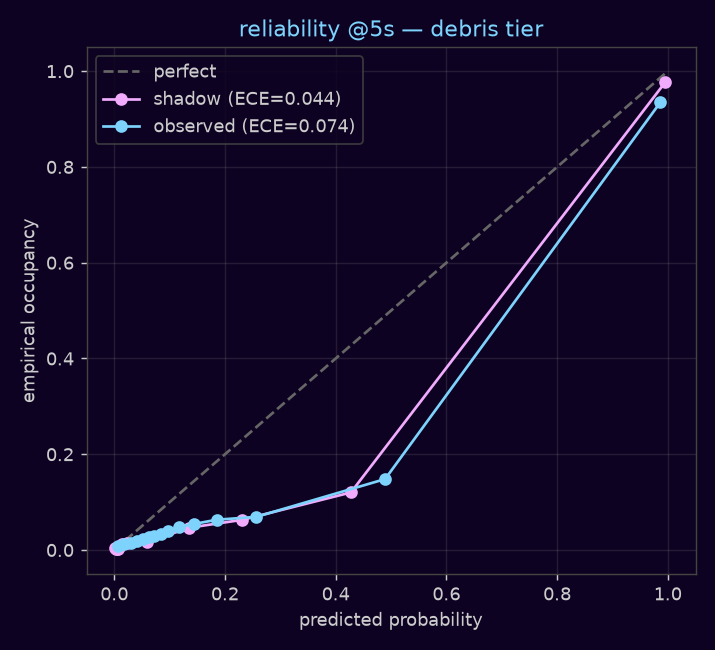
\includegraphics[width=0.55\linewidth]{reliability.png}
  \caption{Reliability diagram restricted to shadow cells (equal-mass binning: a fine 1000-bin
  histogram merged into 15 equal-count macro-bins), debris tier. At 5\,s, in-shadow ECE is
  0.043--0.047 across tiers --- lower than in directly observed space (0.058--0.086) --- with
  Brier 0.022--0.036; the model is underconfident in the mid-range but places little mass there.}
  \label{fig:reliability}
\end{figure}

\end{document}
